\documentclass{article}


% ready for submission
\usepackage[final]{hlt_project_template}
\usepackage{natbib}
\usepackage{float}
\usepackage{graphicx}
\bibliographystyle{plainnat}



\usepackage[utf8]{inputenc} % allow utf-8 input
\usepackage[T1]{fontenc}    % use 8-bit T1 fonts
\usepackage{hyperref}       % hyperlinks
\usepackage{url}            % simple URL typesetting
\usepackage{booktabs}       % professional-quality tables
\usepackage{amsfonts}       % blackboard math symbols
\usepackage{nicefrac}       % compact symbols for 1/2, etc.
\usepackage{microtype}      % microtypography
\usepackage{xcolor}         % colors
\usepackage{amsmath}
\usepackage{tikz}
\usetikzlibrary{positioning}


\title{Trip Advisor Reviews Sentiment Analysis using RNN and Transformers} 


\author{%
  Salvatore Mastrangelo\\
  \texttt{s.mastrangelo4@studenti.unipi.it}
}


\begin{document}


\maketitle


\begin{abstract}
This report presents a comprehensive analysis of sentiment classification on Trip Advisor reviews using 
Recurrent Neural Networks (RNNs) and Transformers. The study explores the effectiveness of these models 
in understanding and predicting sentiment from textual data. A detailed methodology, experimental setup, 
and results are provided, highlighting the strengths and weaknesses of each approach. In particular,
given a rather small dataset of Trip Advisor reviews, the aim is to classify the sentiment of each review into both
stars classes (1 to 5 stars) and ternary classes (positive, negative, neutral). RNN models are implemented
using Long Short-Term Memory (LSTM), while Transformers are implemented using the BERT architecture, in
particular the RoBERTa model. The results show that while Transformers require much less epochs to 
converge, RNNs are able to achieve better performance in terms of accuracy and F1 score on such
small dataset. On the other hand, Transformers show much better capabilities in terms of ambiguous reviews, 
achieving a better F1 score and accuracy in the middle part of the scale (3-4 stars). 
\end{abstract}

\section{Introduction}
\label{sec:introduction}
    \subsection{Nature of sentiment analysis}
    \label{subsec:nature_of_sentiment_analysis}
        Sentiment Analysis is a subfield of Natural Language Processing (NLP) that focuses on identifying
        and classifying subjective information in text data. In particular, it allows to cathegorize the
        sentiment expressed by pieces of text, such as reviews, comments, or social media posts, into 
        predefined classes, that can be whether:
        \begin{itemize}
            \item favorable or unfavorable opinions towards a product, service, or entity,
            \item expressed emotions such as joy, anger, sadness, or fear,
            \item opinions about specific aspects or features of a product or service (aspect-based sentiment).
        \end{itemize}
        Sentiment analysis is widely used in various domains, including marketing, customer service, 
        and social media, to gain insights into public opinion or provide control over allowed content,
        like in the case of hate speech detection.

    \subsection{Approaches to Sentiment Analysis}
    \label{subsec:approaches_to_sentiment_analysis}
        The methods used for sentiment analysis can be broadly categorized into: 
        \begin{itemize}
            \item \textbf{Rule-based systems}, which use lexicons and pattern-based approaches, typically hand-crafted,
                    that require large efforts to develop and mantain \citep{gupta2024comprehensivestudysentimentanalysis}.
            \item \textbf{Feature engineering and Machine Learning}, that is based on extraction of features as
                    bag-of-words, n-grams, or word embeddings, followed by machine learning classifiers \citep{gupta2024comprehensivestudysentimentanalysis}.
        \end{itemize}
        In particular, machine learning models have gained in recent years a lot of attention, as recurrent models
        like Long Short-Term Memory (LSTM) networks have shown effective capabilities in capturing relations among
        distant words in a sentence \citep{staudemeyer2019understandinglstmtutorial}, and Transformers like
        BERT \citep{devlin2019bert} and its variants have shown state-of-the-art performance in many NLP tasks.

    \subsection{The project}
    \label{subsec:the_project}
        In this project, the focus is posed on implementation and evaluation two models, one based on LSTM-RNN 
        and one based on RoBERTa \citep{liu2019robertarobustlyoptimizedbert}, a variant of BERT \citep{devlin2019bert},
        that are able to classify the sentiment of hotel reviews, and return a score from 1 to 5 stars, as well
        as a ternary classification of the sentiment expressed, that can be positive, negative or 
        neutral.
\section{Background}
\label{sec:background}
    The background of this project can be divided into two main parts.

    \subsection{models}
    \label{sec:models}
        The first part is about the models used in this project. LSTM-RNNs have been used for
        a long time in Natural Language Processing for its capabilities in capturing long-term
        dependencies among data, overcoming the problem of vanishing gradients that affects RNNs
        \citep{hochreiter1997long}. Such models implement a memory cell that can block or allow
        the flow of information from the past to the future using three gates:
        input, forget and output gates.\\
        
        Some simpler models, like the Gated Recurrent Unit (GRU) \citep{cho2014learning},
        have been proposed to reduce the number of parameters, but still keeping the
        same concept of memory cell. Both LSTM and GRU have been widely used and
        show strenghts in different tasks, with LSTM being more suitable for
        higher-complexity sequencies and GRU for simpler ones \citep{Cahuantzi_2023} \\

        Transformers, on the other hand, are a more recent architecture \citep{vaswani2023attentionneed}
        that has revolutionized the field of sequence processing and thus Natural
        Language Processing, that uses self-attention mechanisms to capture 
        relations among words, allowing parallelization too. \\

        BERT \citep{devlin2019bert} and its variants, like RoBERTa \citep{liu2019robertarobustlyoptimizedbert},
        are pre-trained models that are born from such Transformer architecture used
        as encoders for text data. Trained on large corpora of text, can be 
        fine-tuned on specific tasks to achieve brilliant results with very few 
        variations in the architecture.

    \subsection{related works}
    \label{sec:related_works}
        The second part is about the related works in the field of sentiment analysis.
        Many works have been done in the past, using different approaches and models,
        but the most recent ones focus on the use of Transformers and pre-trained models
        like BERT and its variants.\\
        
        In particular, \citet{gupta2024comprehensivestudysentimentanalysis} provide a comprehensive
        study on sentiment analysis, comparing different approaches and models, including
        rule-based systems, machine learning classifiers, and deep learning models like LSTM
        and Transformers. They highlight the strengths and weaknesses of each approach,
        showing that while rule-based systems can be effective for specific tasks, machine learning
        and deep learning models are more suitable for general-purpose sentiment analysis.\\
        
        An interesting work is done by \citet{wen2023sentiment}, who provides a
        similar study on sentiment analysis using another variant of BERT, called
        ERNIE, that uses knowledge graphs to improve the understanding of language
        structure and semantics. They show that ERNIE outperforms BERT in various
        knowledge-intensive tasks, while retaining comparable performance in 
        other NLP tasks. \citep{zhang2019ernieenhancedlanguagerepresentation}
\section{Methods}
\label{sec:methods}    
    In this section the methodologies implemented are illustrated, starting from the
    dataset used, the preprocessing steps and the models implemented.

    \subsection{Dataset}
    \label{subsec:dataset}
        The dataset used in this project is a collection of Trip Advisor reviews, taken
        from kaggle\footnote{\url{https://www.kaggle.com/datasets/andrewmvd/trip-advisor-hotel-reviews}}.
        Such dataset contains 20491 english reviews of hotels, labelled with a score from
        1 to 5 stars (labels 0 to 4). To grant a more balanced benckmark, all the reviews with a
        length greater than 256 tokens according to the RoBERTa tokenizer were 
        dropped, resulting in a final dataset of 18273 reviews. Such choice was
        made to make a compromise between the maximum depth of the LSTM Networks
        in order to avoid vanishing gradients, and the maximum length of the
        \textit{roberta\_base} tokenizer and model, which is 512 tokens. Then, some preprocessing
        steps were done, such as removing HTML tags, converting the reviews to 
        lowercase and removing stop words according to the NLTK default list. 
        The final distribution of labels is the following:
        \begin{figure} [H]
            \centering
            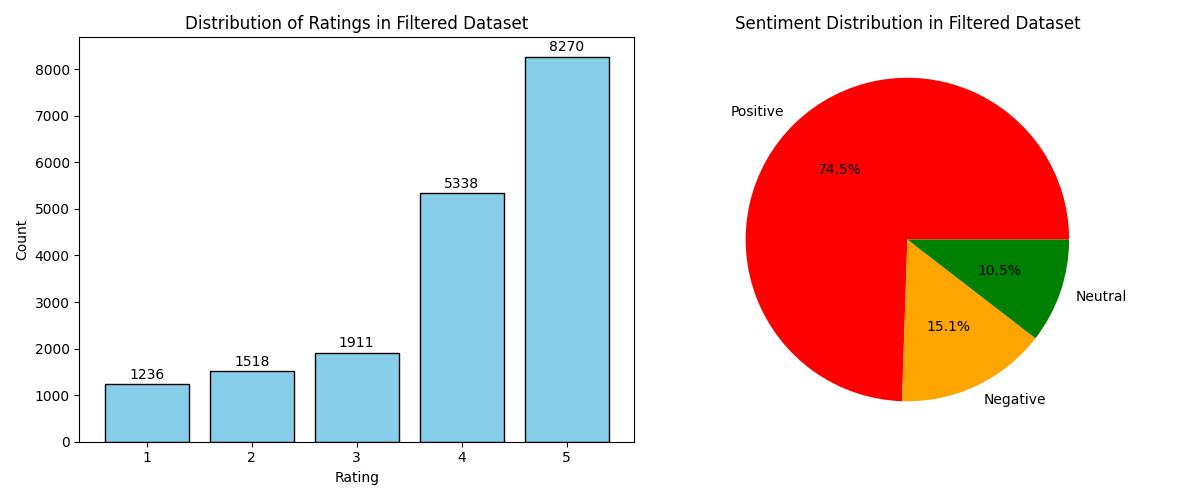
\includegraphics[width=\textwidth]{images/label_distribution.png}
            \caption{Label distribution}
        \end{figure}
        The dataset is quite unbalanced, with a vast majority of positive reviews (4-5 stars). 

        The reviews were then split into:
        \begin{itemize}
            \item training set: $72.3\%$
            \item validation set: $12.7\%$
            \item test set: $15\%$
        \end{itemize}

        Based on the used model, the reviews were converted to tokens either using The
        RoBERTa tokenizer, either using the NLTK tokenizer, which was used to create the
        vocabulary for the RNN model. Both tokenized datasets were then padded to a maximum 
        length of 256 tokens.

    \subsection{Models}
    \label{subsec:models}
        \subsubsection{LSTM-RNN}
        \label{subsubsec:lstm}
            The first model implemented is a Long Short-Term Memory (LSTM) Recurrent
            Neural Network (RNN) implemented in Torch, made of:
            \begin{itemize}
                \item an embedding layer, which converts the input tokens to a dense vector representation;
                \item a LSTM layer, which processes the sequence of embeddings and captures the sequence temporal dependencies;
                \item a fully connected layer, which maps the output of the LSTM to the final output classes.
                \item a softmax activation function
            \end{itemize}

            \begin{figure}[H]
                \centering
                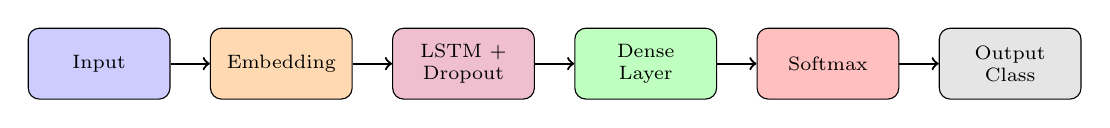
\begin{tikzpicture}[
                    node distance=0.8cm and 0.5cm,
                    every node/.style={align=center, font=\scriptsize},
                    layer/.style={draw, rounded corners, minimum height=0.9cm, minimum width=1.8cm, text centered},
                    input/.style={layer, fill=blue!20},
                    embed/.style={layer, fill=orange!30},
                    lstm/.style={layer, fill=purple!25},
                    dense/.style={layer, fill=green!25},
                    softmax/.style={layer, fill=red!25},
                    output/.style={layer, fill=gray!20}
                ]

                    % Nodes (horizontal layout)
                    \node (input) [input] {Input};
                    \node (embedding) [embed, right=of input] {Embedding};
                    \node (lstm) [lstm, right=of embedding] {LSTM + \\ Dropout};
                    \node (fc) [dense, right=of lstm] {Dense \\ Layer};
                    \node (sm) [softmax, right=of fc] {Softmax};
                    \node (out) [output, right=of sm] {Output \\ Class};

                    % Arrows
                    \draw[->, thick] (input) -- (embedding);
                    \draw[->, thick] (embedding) -- (lstm);
                    \draw[->, thick] (lstm) -- (fc);
                    \draw[->, thick] (fc) -- (sm);
                    \draw[->, thick] (sm) -- (out);

                \end{tikzpicture}
                \caption{LSTM-based sentiment classifier.}
            \end{figure}

            In particular, to evaluate the performance of the model, only the
            higher probability class is selected.
            The model is trained using the ADAM optimizer \citep{kingma2017adam},
            based on the cross-entropy loss function. Some form of dropout
            is applied to the LSTM layer to avoid overfitting.
            the model is trained for a maximum of 100 epochs, with early stopping
            kicking in almost always before the epochs upper limit, based on the 
            accuracy on the validation set.
            Ultimately, the hyperparameters used for the model are: \\
            (\textbf{bold} values are the chosen ones)
            \begin{table}[H]
                \centering
                \begin{tabular}{l c c c}
                    \toprule
                    \multicolumn{1}{l}{\textbf{Hyperparameter}} & \multicolumn{3}{c}{\textbf{Values}} \\                  \midrule
                    Dropout & 0 & 0.1 & \textbf{0.3} \\
                    Learning rate & 0.001 & 5e-4 & \textbf{3e-4} \\
                    Patience & 0 & \textbf{5} & 10 \\
                    \bottomrule
                \end{tabular}
                \label{tab:lstm_hyperparams}
            \end{table}
            The tokenizer used in this model, as said before, is the NLTK tokenizer,
            with a vocabulary size of 10002, corresponding to the 10000 most
            frequent words in the training set, plus the \texttt{<PAD>} and \texttt{<OOV>} tokens,
            corresponding to the padding token and the out-of-vocabulary token.


        \subsubsection{RoBERTa Transformer}
        \label{subsubsec:roberta}
            The second model implemented is a RoBERTaForSequenceClassification transformer
            from the HuggingFace Transformers library, initialized at the \textit{roberta-base} 
            checkpoint. Furthermore, a classification MLP head is present, that takes information 
            from the first output of the RoBERTa transformer, which corresponds to the 
            \texttt{[CLS]} token, and maps it to the final output classes using softmax activation.

            \begin{figure}[H]
                \centering
                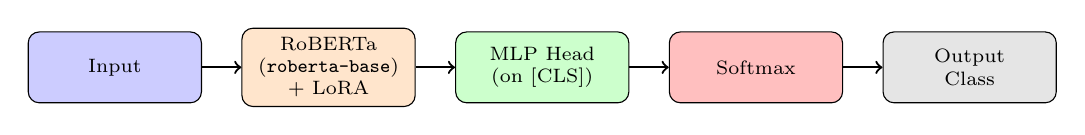
\begin{tikzpicture}[
                    node distance=0.8cm and 0.5cm,
                    every node/.style={align=center, font=\scriptsize},
                    layer/.style={draw, rounded corners, minimum height=0.9cm, minimum width=2.2cm, text centered},
                    input/.style={layer, fill=blue!20},
                    roberta/.style={layer, fill=orange!20},
                    mlp/.style={layer, fill=green!20},
                    softmax/.style={layer, fill=red!25},
                    output/.style={layer, fill=gray!20}
                ]

                    % Nodes (horizontal layout)
                    \node (input) [input] {Input};
                    \node (encoder) [roberta, right=of input] {RoBERTa\\(\texttt{roberta-base}) \\ + LoRA};
                    \node (mlp) [mlp, right=of encoder] {MLP Head\\(on [CLS])};
                    \node (sm) [softmax, right=of mlp] {Softmax};
                    \node (out) [output, right=of sm] {Output \\ Class};

                    % Arrows
                    \draw[->, thick] (input) -- (encoder);
                    \draw[->, thick] (encoder) -- (mlp);
                    \draw[->, thick] (mlp) -- (sm);
                    \draw[->, thick] (sm) -- (out);

                \end{tikzpicture}
                \caption{RoBERTa-based sentiment classifier.}
            \end{figure}

            The model, even though is pretrained, is fine-tuned on the datset using a rank-32 LoRA (Low-Rank Adaptation) PEFT
            with dropout. Like with the LSTM-RNN model the training has place using the cross-entropy loss function, 
            with the optimization performed using the ADAMW optimizer \citep{loshchilov2019decoupledweightdecayregularization}
            It should be noted that the model is trained using fp16 mixed precision, allowing
            to speed up the training and reducing the memory usage, allowing the
            training of the model on a single GPU with 6GB of memory.
            The final hyperparameters used for the model are: \\
            (\textbf{bold} values are the chosen ones)
            \begin{table}[H]
                \centering
                \begin{tabular}{l c c c}
                    \toprule
                    \multicolumn{1}{l}{\textbf{Hyperparameter}} & \multicolumn{3}{c}{\textbf{Values}} \\                  \midrule
                    LoRA Dropout & 0 & \textbf{0.1} & 0.3 \\
                    LoRA Alpha & 16 & \textbf{32} & 64 \\
                    Learning rate & 1e-5 & 2e-5 & \textbf{3e-5} \\
                    \bottomrule
                \end{tabular}
                \label{tab:roberta_hyperparams}
            \end{table}
            Furthermore, a Learning Rate Warmup \citep{kalra2024warmuplearningrateunderlying} of 10\% of the training steps
            is applied.
            The tokenizer used in this model is the \textit{roberta-base} tokenizer.
\section{Experimental analysis}
\label{sec:experimental_analysis}
    \subsection{Task}
      \label{sec:task}
        As mentioned in the introduction, the task consists in classifying sentences
        based on the sentiment expressed by them. after the training of the models,
        the desired output is a class, in the range from 1 to 5 stars in the first place,
        and in the range [0, 2] in the second place, where 0 is negative, 1 is neutral and
        2 is positive. \\
        
        Furthermore, such task is performed with the purpoose of not only gather 
        metrics about the generalization capabilities of the architectures implemented,
        but also to compare the performance of the two.
      

    \subsection{Experimental settings}
    Describe all the relevant aspects of the experimental setup used in your 
    experiment (e.g., how you performed model selection for fine-tuning of 
    hyper-parameters, all details regarding the learning / fine-tuning of your 
    model, etc.)
    \subsection{Results} 
    Provide results (figures and tables with mounerical results should go here). 
    Provide insights and comments on the achieved results (also comparatively with literature). Possible ablation studies go here.
\section{Discussion}
Overall discussion on the results, relevant insights.
Frame your considerations in the current landscape of relevant research.
\section{Conclusions}
Draw conclusions and possibly delineate future works / possible improvements.

\bibliography{bib.bib}

\small

%%%%%%%%%%%%%%%%%%%%%%%%%%%%%%%%%%%%%%%%%%%%%%%%%%%%%%%%%%%%

\appendix

\section{Appendix / supplemental material}


Optionally include supplemental material (complete proofs, additional experiments and plots) in appendix.

\end{document}